\documentclass{beamer}
\usepackage{ArmenianSlides}

\begin{document}

\title[Bridge]{Նախագծման Ձևանմուշներ։ Bridge}
\author[Հրաչյա Թանդիլյան\copyright]{Հրաչյա Թանդիլյան}
\date{2020}

%-------------------------------------------------------------------------------------------------
\begin{frame}
\titlepage
\end{frame}
%-------------------------------------------------------------------------------------------------

\section{Նպատակը}
%-------------------------------------------------------------------------------------------------
\begin{frame}\frametitle{Bridge}
\begin{block}{Նպատակը}
    Առանձնացնում է աբստրակցիան (ինտերֆեյսը) իրականացումից այնպես,
    որ այդ երկուսը կարող են փոփոխվել միմյանցից անկախ:
\end{block}
\vfill
Նաև հայտնի է որպես
\begin{itemize}
    \item Handle / Body
\end{itemize}
\end{frame}
%-------------------------------------------------------------------------------------------------

\subsection{Մոտիվացիան}
%-------------------------------------------------------------------------------------------------
\begin{frame}\frametitle{Մոտիվացիան}
\begin{center}
    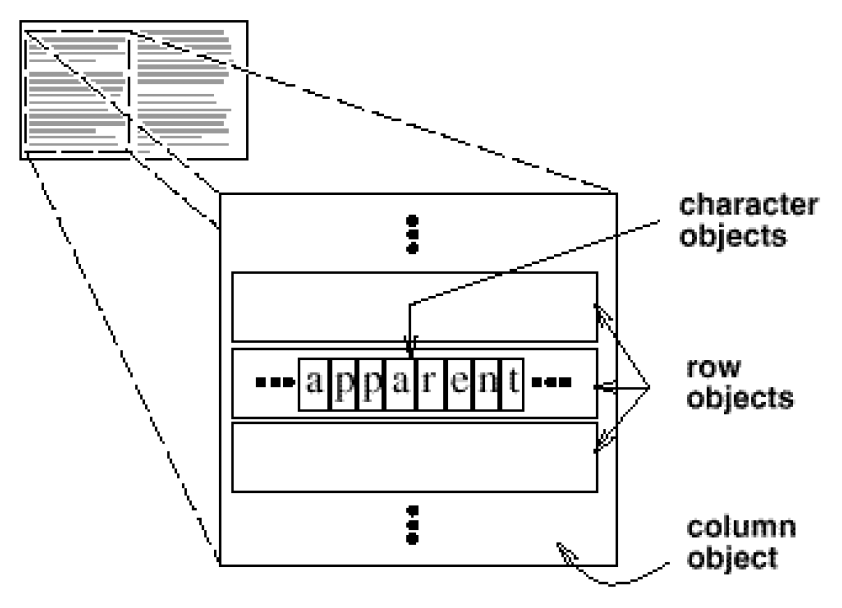
\includegraphics[scale=0.4]{motivation1.png}
\end{center}
\end{frame}
%-------------------------------------------------------------------------------------------------

%-------------------------------------------------------------------------------------------------
\begin{frame}\frametitle{Մոտիվացիան}
\begin{center}
    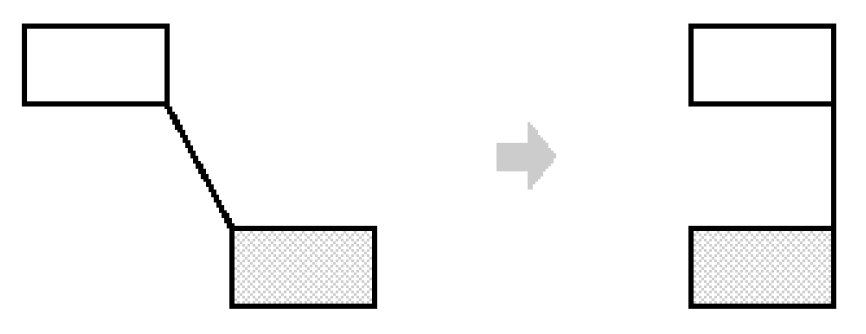
\includegraphics[scale=0.4]{motivation2.png}
\end{center}
\end{frame}
%-------------------------------------------------------------------------------------------------

\subsection{Կիրառելիությունը}
%-------------------------------------------------------------------------------------------------
\begin{frame}\frametitle{Կիրառելիությունը}
Այս Ն.Ձ. պետք է օգտագործել երբ.
\vfill
{
    \scriptsize
    \begin{enumerate}
        \item Անհրաժեշտ է աբստրակցիաի և իրականացման մեջ մշտական
        կապ չստեղծել: \pause \vfill
        \item և՛ աբստրակցիան, և՛ իրականացումը պետք է ընդլայնելի լինեն
        ժառանգության միջոցով: \pause \vfill
        \item Աբստրակցիաի իրականացման մեջ փոփոխությունները օգտագործողների
        վրա չպետք է ազդեցություն ունենան, այսինքն նրանց կոդը չպետք է
        վերակոմպիլիացիաի ենթարկվի: \pause \vfill
        \item (C++) Անհրաժեշտ է աբստրակցիաի իրականացումը ամբողջովին թաքցնել
        օգտագործողներից: \pause \vfill
        \item Անհրաժեշտ է միևնույն իրականացումը օգտագործել մի քանի օբյեկտների
        համար և այդ փաստը պետք է թաքնված լինի օգտագործողից:
    \end{enumerate}
}
\end{frame}
%-------------------------------------------------------------------------------------------------

\section{Կառուցվածքը}
%-------------------------------------------------------------------------------------------------
\begin{frame}\frametitle{Կառուցվածքը}
\begin{center}
    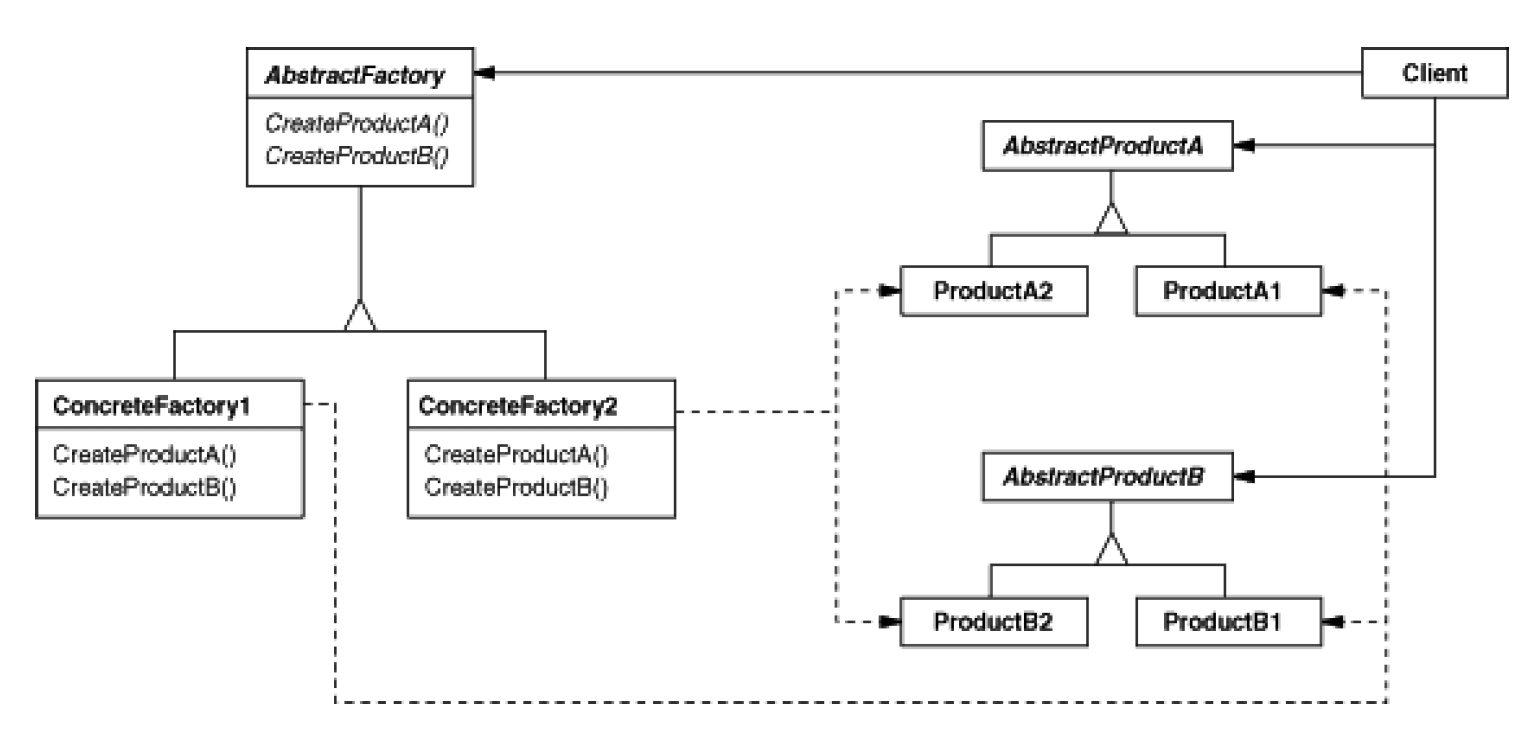
\includegraphics[scale=0.4]{structure.png}
\end{center}
\end{frame}
%-------------------------------------------------------------------------------------------------

\subsection{Հետևանքները}
%-------------------------------------------------------------------------------------------------
\begin{frame}\frametitle{Հետևանքները}
Այս Ն.Ձ. ունի հետևյալ առավելություններն ու թերությունները.
\vfill
\begin{enumerate}
    \item Բաժանում է ինտերֆեյսը իրականացումից: \pause \vfill
    \item Բարելավում է ընդլայնելիությունը: \pause \vfill
    \item Իրականացման մանրամասները քողարկում է օգտագործողից:
\end{enumerate}
\end{frame}
%-------------------------------------------------------------------------------------------------

\section{Իրականացումը}
%-------------------------------------------------------------------------------------------------
\begin{frame}\frametitle{Իրականացումը}
\begin{enumerate}
    \item Միայն մեկ իրականացում: \vfill
    \item Համապատասխան իրականացնող օբյեկտի ստեղծում: \vfill
    \item Ընդհանուր իրականացնող օբյեկտների կիրառում: \vfill
    \item Բազմակի ժառանգության կիրառում:
\end{enumerate}
\end{frame}
%-------------------------------------------------------------------------------------------------

\subsection{Օրինակ}
%-------------------------------------------------------------------------------------------------
\begin{frame}[fragile]\frametitle{Օրինակ}
\begin{english}
\begin{minted}[fontsize=\scriptsize]{cpp}
class Window {

public:
    Window(View* contents);
    virtual void DrawContents();
    virtual void Open();                       // Close();
    virtual void Iconify();                    // Deiconify();
    virtual void SetOrigin(const Point& at);
    virtual void SetExtent(const Point& extent);
    virtual void DrawRect(const Point&, const Point&);
    // DrawLine, DrawPolygon, DrawText

protected:
    WindowImp* GetWindowImp();
    View* GetView();

private:
    WindowImp* imp;
    View* contents;
};
\end{minted}
\end{english}
\end{frame}
%-------------------------------------------------------------------------------------------------

%-------------------------------------------------------------------------------------------------
\begin{frame}[fragile]\frametitle{Օրինակ}
\begin{english}
\begin{minted}{cpp}
class WindowImp {

public:
    virtual void ImpTop() = 0;
    virtual void ImpBottom() = 0;
    virtual void ImpSetExtent(const Point&) = 0;
    virtual void ImpSetOrigin(const Point&) = 0;

    virtual void DeviceRect(Coord, Coord, Coord, Coord) = 0;
    virtual void DeviceText(const char*, Coord, Coord) = 0;
    virtual void DeviceBitmap(const char*, Coord, Coord) = 0;
    // more functions for drawing on windows

protected:
    WindowImp();
};
\end{minted}
\end{english}
\end{frame}
%-------------------------------------------------------------------------------------------------

%-------------------------------------------------------------------------------------------------
\begin{frame}[fragile]\frametitle{Օրինակ}
\begin{english}
\begin{minted}{cpp}
WindowImp* Window::GetWindowImp() {

    if (imp == 0) {
        imp = WindowSystemFactory::Instance()->MakeWindowImp();
    }
    return imp;
}

void Window::DrawRect(const Point& p1, const Point& p2) {

    WindowImp* imp = GetWindowImp();

    imp->DeviceRect(p1.X(), p1.Y(), p2.X(), p2.Y());
}
\end{minted}
\end{english}
\end{frame}
%-------------------------------------------------------------------------------------------------

%-------------------------------------------------------------------------------------------------
\begin{frame}[fragile]\frametitle{Օրինակ}
\begin{english}
\begin{minted}[fontsize=\scriptsize]{cpp}
class ApplicationWindow : public Window {

public:
    virtual void DrawContents() {
        GetView()->DrawOn(this);
    }
};

class IconWindow : public Window {

public:
    virtual void DrawContents() {
        WindowImp* imp = GetWindowImp();
        imp->DeviceBitmap(bitmapName, 0.0, 0.0);
    }

private:
    const char* bitmapName;
};
\end{minted}
\end{english}
\end{frame}
%-------------------------------------------------------------------------------------------------

\section{Առնչվող Ձևանմուշները}
%-------------------------------------------------------------------------------------------------
\begin{frame}\frametitle{Առնչվող Նախագծման Ձևանմուշները}
\begin{itemize}
    \item Abstract Factory \vfill
    \item Adapter
\end{itemize}
\end{frame}
%-------------------------------------------------------------------------------------------------

\end{document}
